\section{Selection Efficiencies}
\label{sec:selection}

As a summary of the previous sections, the cut flow of the analysis is as follows:
\begin{itemize}
\item At least two photons and two jets in the event
\item At least two photons pass the trigger based pre-selection (see Sec. \ref{sec:trigger});
\item At least two photons pass the kinematic and identification requirements (see Sec. \ref{sec:photons}) $\to$ select two highest $E_{T}$ photons as diphoton candidate;
\item At least two jets pass the kinematic selection (see Sec.~\ref{sec:jets}) $\to$ select two jets with highest b-tagging score as dijet candidate;
\item Event can be classified in either High Purity Category or Medium Purity Category;
\end{itemize}

The efficiency after each step above and taking into account the acceptance is estimated and shown for each of the signal samples considered in our analysis. 
In Figure \ref{fig:cutflow-res}, the signal efficiency for radions (spin-0) and gravitons (spin-2) from mass hypotheses of 250 up to 900 GeV. 
In Figure \ref{fig:cutflow-nonres}, the signal efficiency for the non-resonant nodes, including top-only contribution (Node 0) and SM (Node 1). 

%We also performed the selection using the cut based photon identification. The ratio of the efficiencies is performed to assess the performance difference between the different photon Id. The result of the comparison is shown in top figure~\ref{fig:cutflow-signal-diff-CutB} and bottom figure~\ref{fig:cutflow-signal-diff-CutB} for Graviton and Radion samples, respectively. The performance of the EGamma MVA photon identification outrates the one of the cut based photon Id., by 10. to 15. \% at low resonance masses, and is around 8-10\% for high resonance masses. \\
%Although we performed a detail study of the MVA photon id. and shown that we could choose a different WP from EGamma MVA(see table~\ref{tab:MVA-WP}), the efficiency for the latter is expectedly  better as shown in figure~\ref{fig:cutflow-signal-diff-MVAEG}.\\
%A comparison of the Graviton and Radion signal efficiencies is also performed in figure~\ref{fig:cutflow-signal-diff-RG}. It is shown that Graviton samples show a better efficiency, more than 10\% higher for high masses.

\begin{figure*}[h]
  \centering
  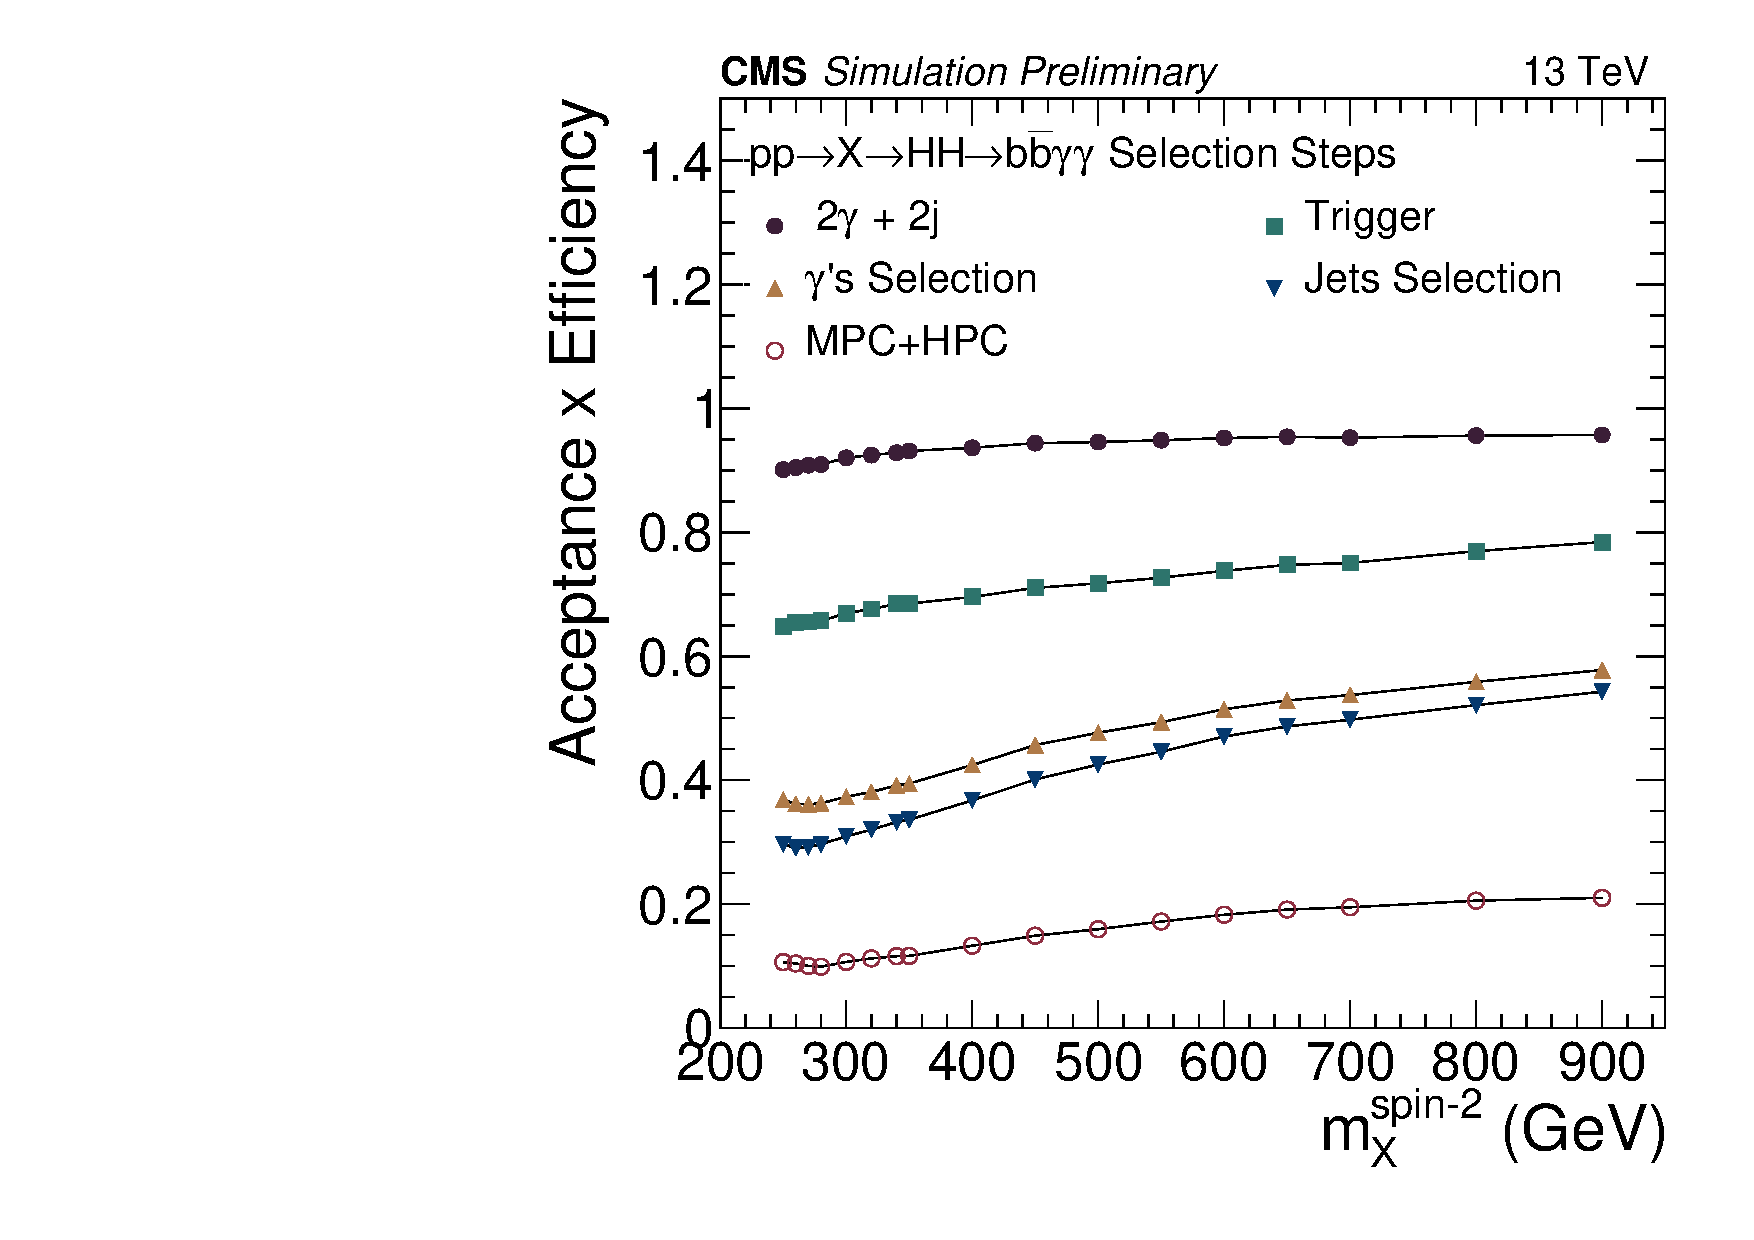
\includegraphics[width=0.45\textwidth]{figures/sec-efficiency_plots/wRegression/res_effs_Graviton_reg.pdf}\hfil
  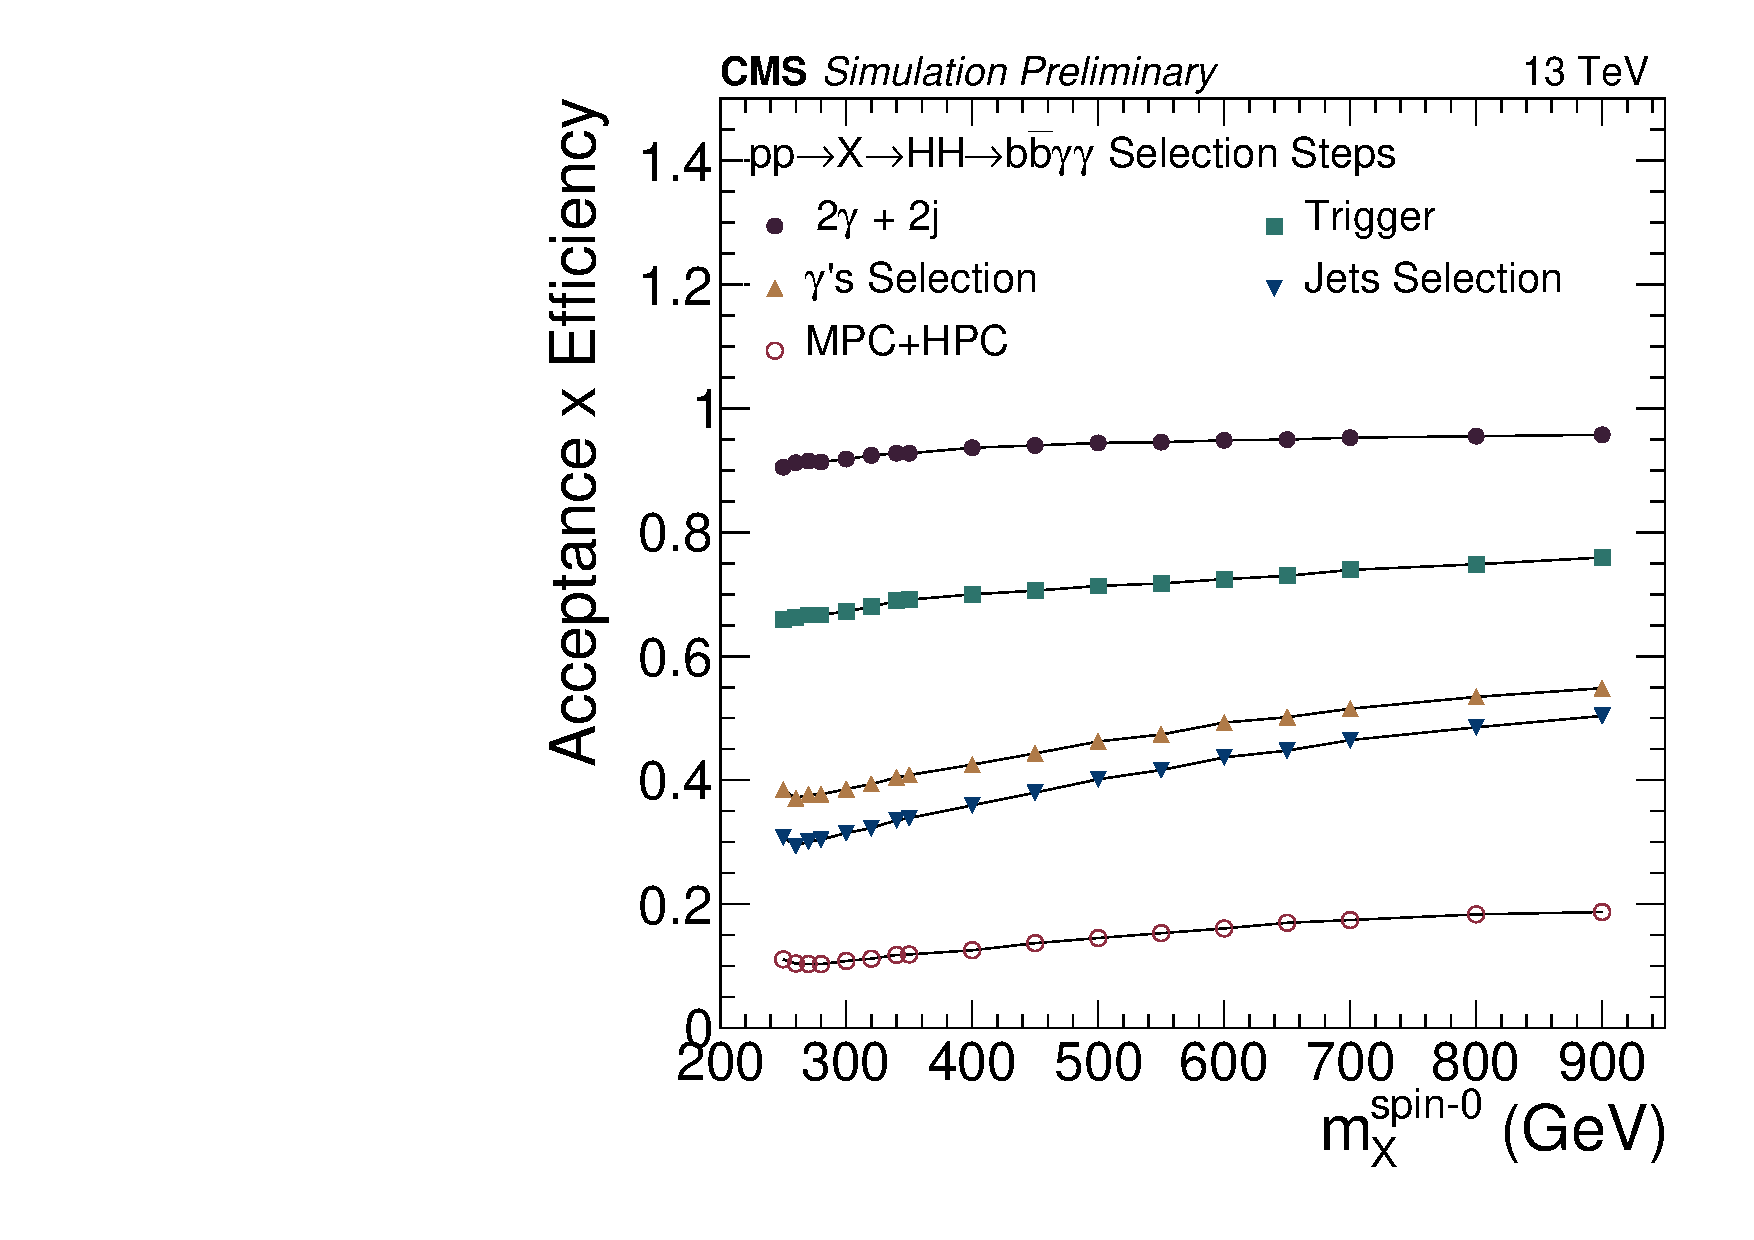
\includegraphics[width=0.45\textwidth]{figures/sec-efficiency_plots/wRegression/res_effs_Radion_reg.pdf}\hfil
  \caption{Graviton (left) and Radion (right) signal acceptance$\times$efficiency for each cut (described in text).}
  \label{fig:cutflow-res}
\end{figure*}

\begin{figure*}[h]
  \centering
  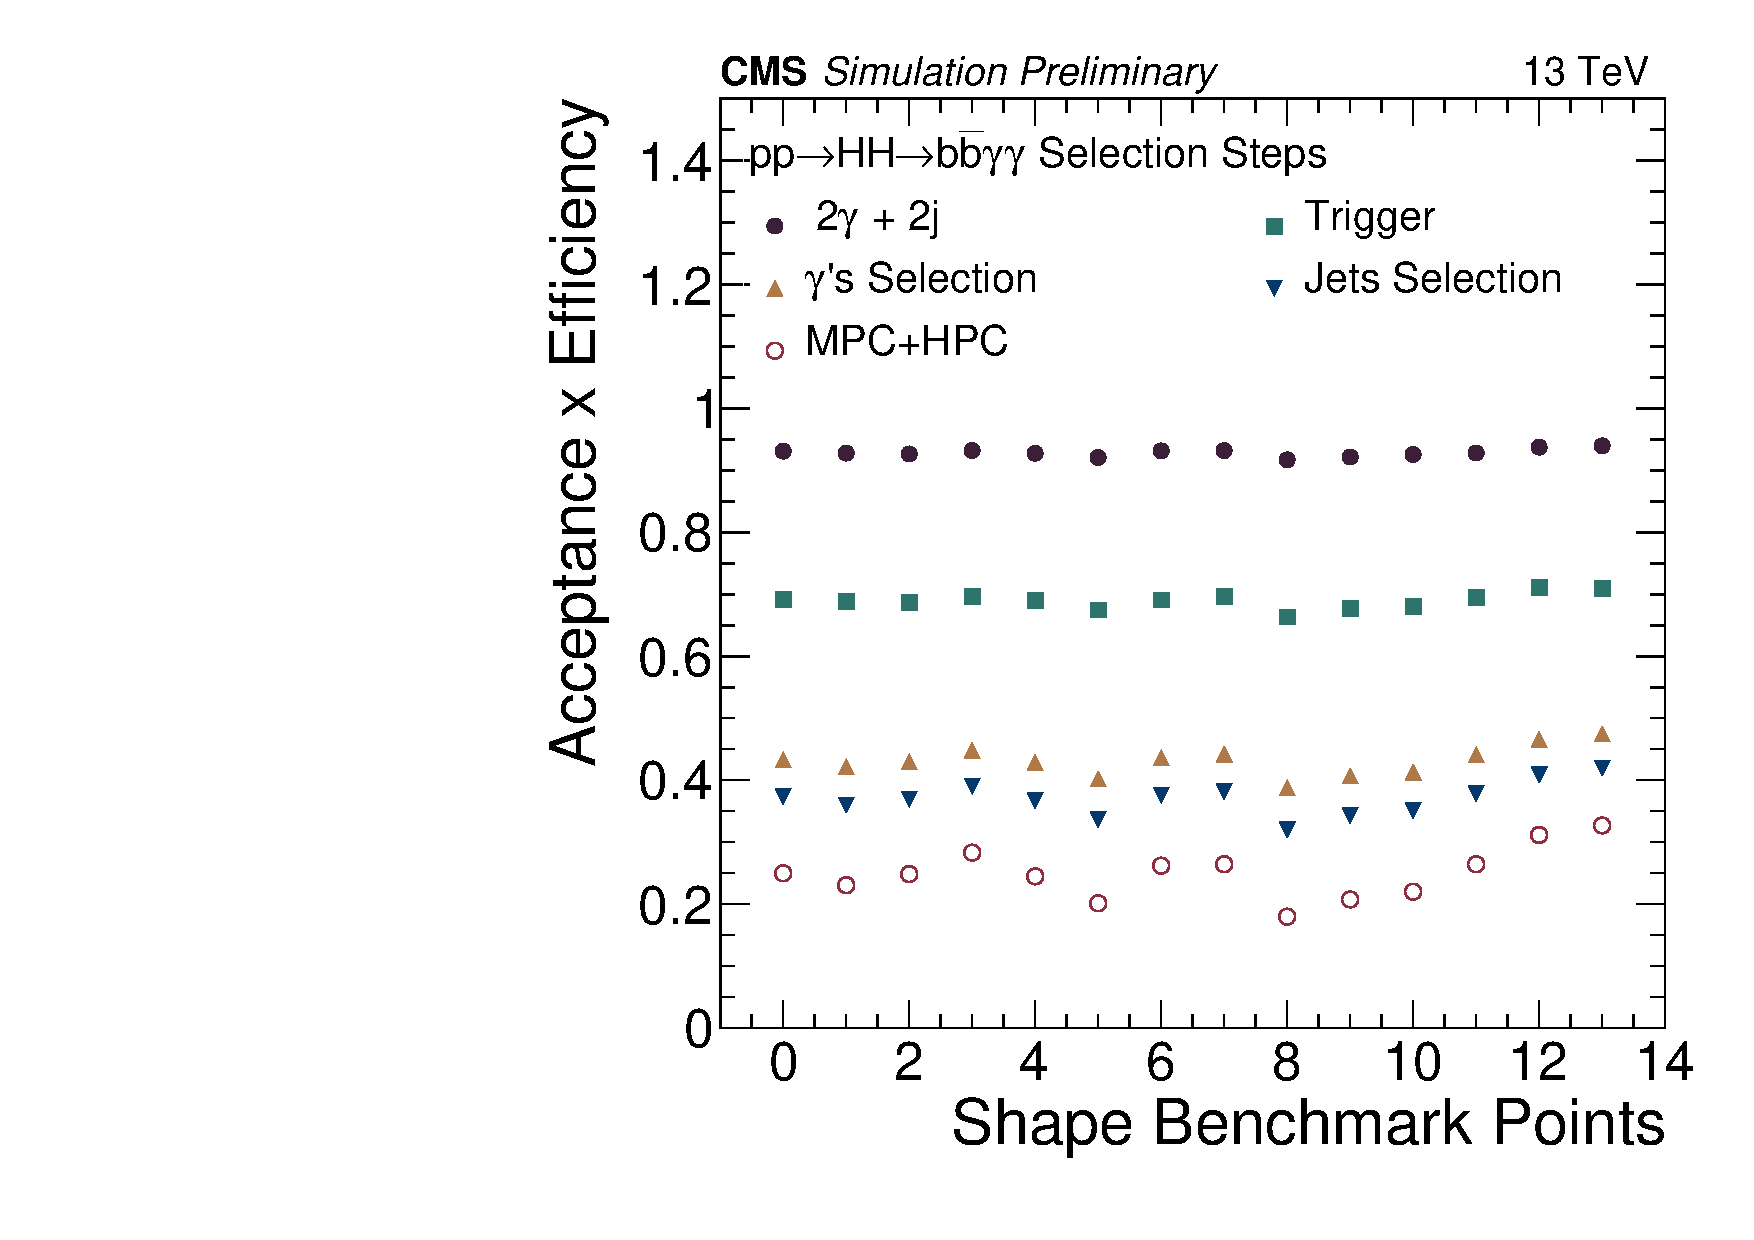
\includegraphics[width=0.45\textwidth]{figures/sec-efficiency_plots/wRegression/nonres_effs_reg.pdf}\hfil
  \caption{Non-resonant acceptance x efficiency. Jet energy regression applied in addition to MVA based categorization.}
  \label{fig:cutflow-nonres}
\end{figure*}


